\documentclass[]{article}
\usepackage{multicol}
\usepackage[margin = 1.25in]{geometry}
\usepackage{graphicx}
\usepackage{mathtools}
\usepackage{caption}
\usepackage{lipsum}
\usepackage{algpseudocode}
\usepackage{fancyvrb}
\usepackage{amsfonts}
\usepackage{amsmath}
\usepackage{textcomp}
\newenvironment{Figure}
  {\par\medskip\noindent\minipage{\linewidth}}
  {\endminipage\par\medskip}

\usepackage{setspace}
\linespread{2.0}
\setlength{\parskip}{1em}

\newtheorem{theorem}{Theorem}[section]
\newtheorem{lemma}[theorem]{Lemma}
\newtheorem{proposition}[theorem]{Proposition}
\newtheorem{corollary}[theorem]{Corollary}

\newenvironment{proof}[1][Proof]{\begin{trivlist}
\item[\hskip \labelsep {\bfseries #1}]}{\end{trivlist}}
\newenvironment{definition}[1][Definition]{\begin{trivlist}
\item[\hskip \labelsep {\bfseries #1}]}{\end{trivlist}}
\newenvironment{example}[1][Example]{\begin{trivlist}
\item[\hskip \labelsep {\bfseries #1}]}{\end{trivlist}}
\newenvironment{remark}[1][Remark]{\begin{trivlist}
\item[\hskip \labelsep {\bfseries #1}]}{\end{trivlist}}

\newtheorem{hyp}{Hypothesis}

\makeatletter
\newcounter{subhyp} 
\let\savedc@hyp\c@hyp
\newenvironment{subhyp}
 {%
  \setcounter{subhyp}{0}%
  \stepcounter{hyp}%
  \edef\saved@hyp{\thehyp}% Save the current value of hyp
  \let\c@hyp\c@subhyp     % Now hyp is subhyp
  \renewcommand{\thehyp}{\saved@hyp\alph{hyp}}%
 }
 {}
\newcommand{\normhyp}{%
  \let\c@hyp\savedc@hyp % revert to the old one
  \renewcommand\thehyp{\arabic{hyp}}%
} 
\makeatother


%opening
\title{Modeling Network User Behavior: Various Approaches}
\date{May 20, 2016}
\author{Shidan Xu}


\begin{document}
\maketitle

%\begin{abstract}
%
%\end{abstract}



\begin{abstract}

This project involves learning to predict users' mobility within the network topology. Topological mobility, as opposed to physical mobility, can be substantial as a user switches from LTE to wifi network, while moving minimally physically. Our dataset consists of email IMAP logs as they document associated client IP addresses, as well as the clients' identifiers. Prediction for online mobility is of particular interest to the networks community. If we can predict online mobility with high probability, then new network architecture can be designed to optimize the caching system by minimizing resending packets.  We used various approaches and techniques to model the user's behavior, including probabilistic programming, regression, neural nets, and clustering algorithms. We compare and contrast how models differ in their prediction accuracy, speed of convergence, and algorithmic complexity. 


\end{abstract}
%This paper describes a thesis project at the MIT Advanced Networks Architecture (ANA) group. This project involves predicting a user's behavior in various networks. In particular, we are interested in how the user is likely to transition between networks. We plan to design various models to predict the user's behavior, and use various evaluation criteria to understand which model most vividly captures the user's behavior. As a learning experience for our team and me, we employ probabilistic programming (PP) techniques. PP is a way of programming that utilizes existing software packages that include encapsulated methods for the inference step of machine learning. By simplifying the implementation, it allows researchers to focus on models. This project has two main objectives. The first is to design several models to capture one or multiple aspects of a typical user, or a group of users' behavior in a network. The second is to evaluate each model to decide which model is more feasible, and which model is applicable under what situations. Together this project aims to give a better understanding of how network user transitions.


\newpage


\section*{Acknowledgement}

I would like to thank Dr. Karen Sollins for giving me an opportunity to work on this MobilityFirst project for my MEng. I loved my time exploring the intricacies in the datasets and I learned so much in the research process.

I would like to thank Dr. Karen Sollins and Dr. Steven Bauer for their continued advice and insight into conceiving this project and thesis.

I would like to thank Dr. Bauer for his technical help and project focus guidance throughout this project. I'd like to thank Dr. Sollins for all of her help with design decisions and project planning. Without their insights, this project would not have been possible. Their help was invaluable.

I would like to thank the MIT Advanced Networks Architecture (ANA) group for having me carry out this research.
 
I would like to thank Tingtao Zhou, Tianfan Xue, and Zhengli Wang for their help with the statistics concepts and machine learning ideas.

Lastly, I would like to thank my family for all of their support, love, and help in life. 

This project was funded in part under NSF Grant 1413973, "NeTS: Large: Collaborative Research: Location-Independent Networks: Evaluation Strategies and Studies". All code written in this project can be found on Github at All the work can be found on Github at https://github.com/shidanxu/mengvfinal.


\newpage
\singlespacing
\tableofcontents
\newpage
\listoffigures
\listoftables

\doublespacing
\linespread{2.0}
\selectfont

\newpage

\section{Introduction}

\subsection{Project Background}

The Internet is approaching a historic inflection point, with mobile platforms and applications replacing the fixed-host/server model that has dominated the Internet since its inception \cite{mobilityfirst}. This gradual shift produces an opportunity to design a new network focused on mobile users. The problem this thesis investigates is motivated by the MobilityFirst project in the FIND (Future Internet Design) initiative \cite{find}, which asks the question of what the requirements should be for a global network 15 years from now, and how we can build such a network if we are not constrained by the current Internet. 

\subsection{Relations to MobilityFirst}
%NEEDS WORK
The MobilityFirst projects presents several major design goals \cite{mobilityfirst}:

\begin{itemize}
\item
Dynamic hosting to provide scalable network mobility.
\item
The robustness of the wireless transfer medium.
\item
Reinforce network security and privacy for both mobile and wired networks.
\item
Provide context-aware mobile services.
\end{itemize}

Mobile users often switch between different networks (such as cellular and wifi) as they move geographically. Traditional networks such as the Internet were designed more for a static user. In designing a new network that is more suited to the mobile users, we need to evaluate this switching behavior. In this thesis project, we evaluate the user's network transition behavior, in order to understand which users should the new network address. This relates to the first design goal. By providing a clearer understanding of the user behavior, new networks can be designed to configure hosts that is more suitable for the user. One aspect of suitable is to minimize the difference in topological distance and geographical distance. We expand this point next.

\subsection{Current Internet Has Inefficiency in Topological Distance}
Developers of the Internet made some design choices with assumptions. One particular assumption is that network mobility is similar to mobility in geography\cite{jacobson}. However, in real world cases, this assumption is often violated. For example, a phone user could transition from a 4G network to Wi-Fi by walking a few meters in real world, but the network topological distance is long. In extreme cases, the nearest path of two nodes in network topology can traverse opposite coasts of the country. Such design is costly for the user to transition between networks. In designing a new network, one of the focal points is to decrease inconsistency between geographical and topological distance, as packets of information need to be rerouted. The future network needs to address this geographically proximate network change, and decrease this data transfer cost.

\begin{Figure}
 \centering
 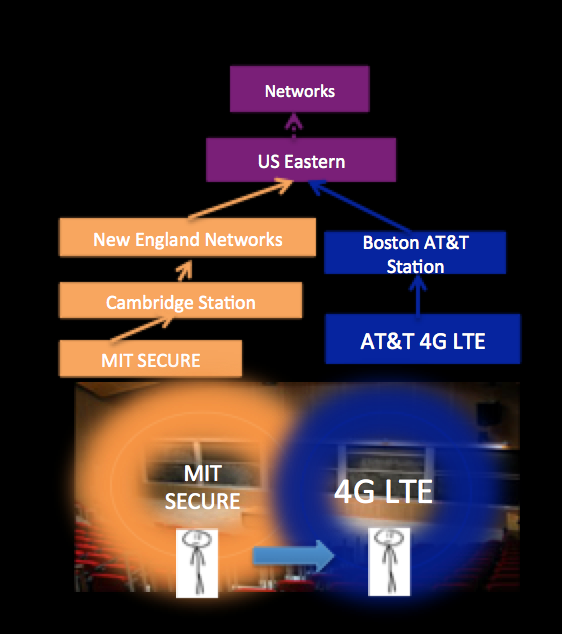
\includegraphics[height = 11cm, width =10cm]{topneqphys.png}
 \captionof{figure}{Physical proximity does not guarantee topological proximity. Small moves in physical space may be large moves in Network topology. The path from the 4G LTE network to the MIT network goes through US Eastern.}
\end{Figure}

Imagine a person traversing through a college campus while checking his email on the phone. As he moves along, his phone's network switches between LTE and his college network alternatively. Every time the user switches network, his phone loses some data and has to send extra requests to recover lost data. The LTE and campus wifi, despite being geographically close by, can be vastly distant in network topology. Hence a request may have to traverse a much longer path than the physically proximity suggests. This extra path traversed slows down packet transfer in the current network. 

Consider another typical 9-5 office worker. She wakes up at 8, goes to work at 9, comes home at 5. She has dinner at 6 and spends two hours surfing the web at night. Now consider how her daily network usage would look like. She would be on her home network in the morning. She uses a combination of the company and LTE network at work. Sometimes she eats lunch at a coffee shop and uses the network there. She spends some time on her home network at night. Her active network traffic ends at 11, but some passive email checking and other maintenance from her device persist throughout the night. Her daily network usage is very predictable. If researchers can predict her network usage, mobile device applications can be customized to make her life more convenient. 

Multiple questions can be asked in those two scenarios. To what accuracy is human network behavior habitual? To what degree can user network behavior be predicted? How should we evaluate network usage behavior? How often do such costly network transitions happen? How do we measure the cost of one such transition? How much traffic is affected by those costly transitions? How should we design our networks to minimize this costly transition?

%%\subsection{A Focus on User Transition Behavior}
%% REVAMPE THIS PARAGRAPH FOR CLARITY. WHY NETWORK USAGE

%This project focuses on understanding the users' transition behavior, as opposed to evaluating network usage. Two main reasons support the decision. 1. Networks are designed to advance knowledge across the spectrum of human endeavors\cite{netsfia}, to facilitate daily life, not vice versa. 2. Studying from the networks perspective increases difficulty in discovering mobility. A network can provide information on who is currently utilizing the network, but does not see the user in a chronological perspective, especially whenever s/he is not on this particular network. 

\subsection{Data Analysis Approaches on Networks Problem}

Additionally, the project stresses to create a procedure for fast exploration of new models using approaches such as probabilistic programming and neural nets. These procedures are chosen to quickly expand on the current model. We spent time in evaluating the different modeling techniques and tools for their prediction accuracy, speed of convergence, and algorithmic complexity. 

Noam Chomsky believed that the Merge operation is one of the fundamental differences that separate humans apart from other primates \cite{whyonlyus}. That is, humans can take two abstract concepts and combine them to create scenarios that s/he has never physically experienced. A person can imagine a dinosaur ripping apart an opera stage as long as he understands dinosaurs and opera, despite he has never seen such an event in reality. This Merge ability can induce creativity. Statistical methods and machine learning are trending approaches to extract insight out of the dataset. By applying machine learning strategies to a networks problem, we try to develop new insights that's not traditionally seen.

\newpage

\section{Previous Works on Quantitative Network Measurements}
In this chapter, we review some of the previous works. We reviewed previous works on quantitive models of user transitioning among networks, we evaluate what kind of approaches were taken for networks datasets. We also evaluate new techniques for implementing models.

%DONE SECTION
\subsection{Sookhyun Yang's Three State Markov Model}
%DONE

This thesis seeks to expand the work on Yang's Measurement and Modeling of User Transition Among Networks \cite{yang}. 

Yang's paper created a 3-state Markov model that's evaluated by measuring the distribution of cost function of signaling a network attachment / detachment, using Internet Message Access Protocol (IMAP) logs for email access for the population of University of Massachusetts at Amherst residents \cite{yang}. 

\subsubsection{Choosing the Dataset}
%DONE
A major difficulty in network mobility research is to select a dataset that captures user transitions. Yang argued for three major criteria for selecting a proper dataset\cite{yang}. 

\begin{itemize}
\item
The application should be frequently used by the user to provide a sufficiently large dataset.
\item
The application can be monitored without introducing inconvenience to the user.
\item
The application provides trackable user identification.
\end{itemize}

Therefore, Yang's choice on IMAP logs is a good exploration that satisfies those requirements. We also had several options choosing our datasets.

\begin{itemize}
\item
Use the Yang dataset.
\item
Collect our own email based dataset.
\item
Use mobility datasets from a third party provider who installs apps to track user network usage.
\end{itemize}

If we pick Yang's dataset, we have a leap ahead into what kind of approaches we can take to understand the dataset. More importantly, we save time in acquiring the dataset ourselves, which in Yang's case took four months. We can also collect our own email-based dataset at MIT. In order to extract more information on the user's age, residence, etc., we need to clear privacy controls from the institute. Such data collection can also be time-consuming. Using mobility datasets from a third party is also an option that can provide a feature-rich dataset. We can include identification features for the users, such as age and gender. This is not possible in the IMAP logs due to the way the protocol is setup. However, using data from a third party creates bias towards only the users who are interested in installing the software. We evaluated our options and continued our work based on Yang's datasets as we see areas of improvement on their work.

The Yang dataset identifies a user by an ID that was intentionally anonymized. The dataset specified times when the user logged into an email service, the IP address s/he uses to attach to the network, and times when the server closes the network connection. We see that the raw dataset is large as it contains many entries, but not as feature-rich as each entry contains limited information.

\subsubsection{Comments on Yang's Work}
%DONE

While the paper serves as a decent exploration baseline, we explore alternatives on some aspects, definitions, and assumptions. For instance, the Yang paper collected two datasets. One dataset contains email logs for campus professors and staff members in the fall. Another dataset contains all users across campus over a four month period in winter.  In evaluating the transition costs, Yang assumed all users in the campus wide dataset formed one uniform group. We hypothesized that users form several groups based on their behavioral patterns, and would like to evaluate potentially different user types. We suspect that students would have their preferred time to access emails (night or morning) depending on the course load and personal preferences. Those factors can possible separate the dataset into multiple clusters. 

Another criticism is that the Markov model is simple and not easily expandable to adapt to specific user types. The only independent parameter in this model is the current state the user is in. If another factor is identified to be significant, the entire modeling process needs to restart. We want to avoid such repetitive work in further modeling, by utilizing tools and techniques that facilitate exploration in modeling space.

\subsection{Beverly Applies Machine Learning to Extract Most Important IP Bit for Traffic Congestion}
%DONE
There are many related works in applying machine learning to a networks problem. In Beverly \cite{beverly}, the author described several learning approaches for attacking various networks traffic problems with minimal datasets. In particular, learning was useful in capitalizing on under-utilized information and inferring behavior reliably. Using a hidden Markov model, Beverly was able to predict mean TCP congestion times based on the IP address bits. By using 8 out of the 32 bits, Beverly can predict the mean congestion time accurately to an error of less than 30ms. We take from Beverly's work that statistics and machine learning can provide unique insights into a dataset. By utilizing statistical methods to aid humans in extracting patterns in data, we can improve prediction accuracies. Beverly's paper provides intuition on which learning approaches to use on what type of problem.

\subsection{Probabilistic Programming As a Tool For Fast Modeling}
%DONE
Probabilistic programming is a generative learning approach, and an ongoing research area. Generative learning approaches can analyze complex scenes more richly and flexibly, but have been less widely embraced due to their slow inference speed and problem specific engineering to obtain robust results \cite{kulkarni}. Like a Markov model, generative approaches can learn the optimal parameters for the model. Once the parameters are set, researchers can use the model to generate new data to compare with the observed testing data. One of the trending topics lately in probabilistic programming is in creating a generic inference engine that facilitates optimization of parameters.  This inference engine facilitates code implementation for different models. Many current applications are under development for probabilistic programming \cite{pporg} (See probabilistic-programming.org for a list of existing probabilistic programming systems). Picture and Venture are two notable probabilistic programming languages conceived at MIT. Both languages focus on the development of a general inference engine. With an inference engine, a user can take the benefit of probabilistic models without having the expertise in statistics. We refrained from using those languages as they are alpha versions and are standalone platforms that have higher learning curves. Instead, we explored PyMC3, a stable python package that's written with a general inference engine. We chose this option because we want to explore more models without having to implement the inference methods ourselves \cite{ghah}. 

In Tenenbaum \cite{tenenbaum}, current applications and limitations for probabilistic programming are discussed, with a vision for hierarchical structural learning. In hierarchical structural learning, the algorithm can learn the dependence of variables. That is, not only can the learning algorithm optimize the parameters for the model, it can also learn the most appropriate structure of the model. With enhanced storage capacities and computational cheapness, hierarchical structural learning can facilitate data mining further by saving the scientists time to conceive the more structurally accurate model.

\paragraph{Summary}
In this chapter, we review some of the related previous works. Three works are especially important to us. Yang\cite{yang} created a three-state Markov Model to predict user transition among networks. Beverly\cite{beverly} applied machine learning techniques to various networks problem. Probabilistic programming, a modeling tool that implements an inference engine to facilitate fast modeling, is reviewed.

\newpage


\section{Reproducing Yang Paper Results}
%SECTION DONE
In this chapter, we first reproduce Yang's Markov chain model for user transition prediction. We then evaluate this model to see areas of improvement.

\subsection{A Peek of the Dataset}
%DONE

We acquired processed IMAP datasets from University of Massachusetts. The dataset included the IMAP logs for 7137 campus wide users. The user population was mainly students \cite{yang} and data were taken from December 3, 2013 to Mar 26, 2014.

\begin{Figure}
 \centering
 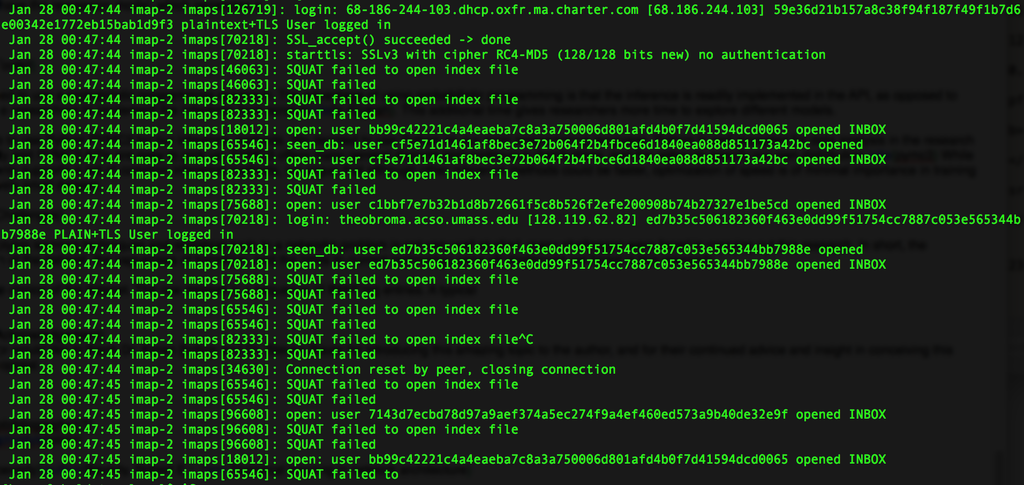
\includegraphics[height = 7cm, width =15cm]{imapSample.png}
 \captionof{figure}{Sample IMAP entry for 2014.01.28}
 \end{Figure}
 
This is what a section of a sample IMAP processed logs file looks like. The most useful information here is that on line 1, a user with an IP address of 68.186.244.103 attached to the network. In the middle section, another user attached to the UMass network. At 00:47:44, the server unilaterally detached the idle user identified by 34630. The log also includes information on when the user checks the inbox and deletes messages. Note that the user identity, which is originally an email address, is masked using SHA2-hashing \cite{yang} to protect user privacy. 

We extract the device the user signed in with, and acquire additional information from the IP address. We used the free website \textit{ip-api.com} to determine the user's city location and internet service provider (ISP) information. We threw out entries that have unidentifiable IP addresses as we used IP addresses to identify when the user is continuously on a network. We did not consider entries with abroad IP addresses because network transition around the world may exhibit different patterns due to the local network infrastructure. Those entries account for roughly 3\% of the entire dataset. 

We note that a user can simultaneously be signed into the same email account from multiple devices or networks. The server does not dismiss a user's first attachment once s/he signs in from a second device.


\subsection{Markov Chain For Transition Prediction}
%DONE
One of the important results in Yang's paper is a 3-state Markov chain model that predicts the likelihood of a user transitioning (defined below), given the number of networks s/he is currently on.

To understand how users make network transitions, first we need to define a transition.

\begin{definition}
A \textbf{session} is a continuous period of time for which a user is on the same network, which is defined by the same IP address. A \textbf{transition} happens when the user detaches from one network and attaches to another one.
\end{definition}

With this definition, we can decide whether a transition happens from the logs. Brian Copeland, a UROP student of the ANA group, parsed the original UMass log entries into entries that contain each individual session. We overlay the durations to decide occurrences of transition. The details of transition criteria can be found in Yang \cite{yang} paper.

A Markov model is a way of modeling the randomly changing systems where the future states only depend on the current state. There are four types of Markov models depending on two criteria. Observable evaluates whether the state of the system is directly observable by the outside. Controlled means for each new step, the system has options on which action to take, and this action affects the transition probabilities. Autonomous means that the system does not have the option to choose an action. 

\begin{center}
    \begin{tabular}{| l | l | l |}
    \hline
     Dimension& System State Fully Observable & System State Partially Observable \\ 
    \hline
    System is Autonomous & Markov Chain &Hidden Markov Model(HMM)\\ 
    System is Controlled& Markov Decision Process(MDP) &Partially Observable MDP\\ 
    \hline
    \end{tabular}
\captionof{table}{Different kinds of Markov Models\cite{markov}}
\end{center}

In Yang, the researchers implemented a Markov Chain, that is, a system with fully observable states and no action options. The three states of the Markov chain are 

\begin{itemize}
\item
On 0 networks
\item
On 1 network
\item
On $\geq 2$ networks
\end{itemize}

A 3 by 3-state transition probability matrix can be calculated directly from the dataset. One subtle choice we have to make is how often we call each time step. One extreme is to take near-continuous measurements. For instance, we can consider every second as a new time step. However, this creates a nearly inescapable state. On average, a typical user logs 20 sessions a day. There are 86400 seconds in one day. This is at most 20/86400 = 0.23\textperthousand. Hence we are likely to be stuck in the on 0 networks state. Using such a model, we might create a skewed dataset that does not faithfully captures the original distribution.

We took measurements at the end of each 20-minute period as Yang concluded 20-minute periods was appropriate for this dataset \cite{yang}. We look at the networks the user is on at the end of the 20-minute window, versus at the beginning, to see whether s/he has transitioned. In table 2, we have the transition probability matrix calculated on a 10000 user days training sample. Given this transition probability matrix, we can generate estimations of what the user may behave in the future. We then compare this model generated data with the testing sample.

\begin{center}
    \begin{tabular}{| l | l | l | l |}
    \hline
     Transition Prob.& On 0 Networks & On 1 Network & On $>=1$ Networks\\ 
    \hline
    On 0 Networks CRF& 0.930 &0.066 & 0.004\\ 
    On 1 Network& 0.696 &0.266 & 0.038\\ 
    On $>=1$ Networks & 0.291 & 0.356 & 0.353\\
    \hline
    \end{tabular}
\captionof{table}{Empirical estimates of transition probabilities. Data acquired on training sample (10000 user days).}
\end{center}

\subsection{Evaluate Markov Chain Prediction}
%DONE
For baseline, we evaluate the distribution of the number of transitions for all users on a daily basis as noted in Yang. We identify a transition as a change of state (on 0, on 1, or on 2 or more) from the end of the previous 20-minute period to the end of the current 20-minute period. We compute one distribution from the testing dataset, and another for the randomly generated dataset based on Markov chain runs. Further, we also included the distribution for the training data we used to produce the transition probability matrix. We make the simple assumption that all users behave similarly. 

\begin{Figure}
 \centering
 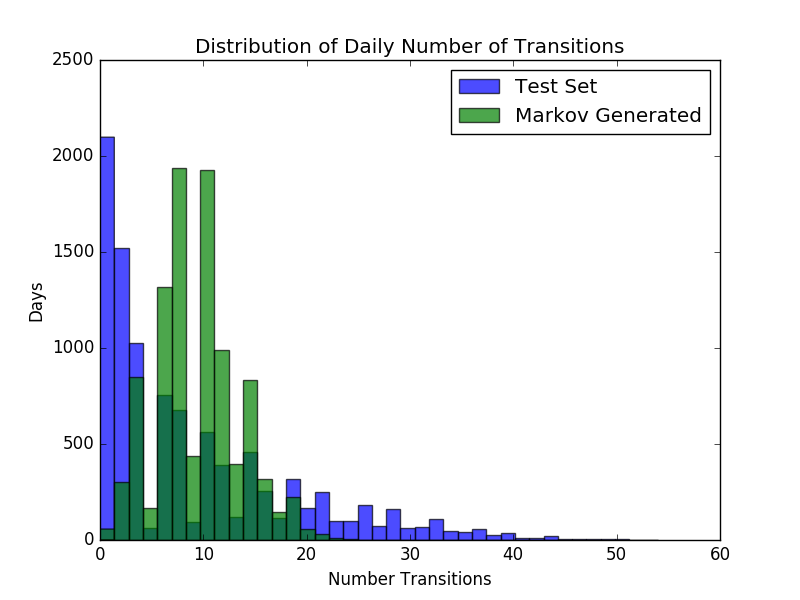
\includegraphics[height = 11cm, width =15cm]{markovGenTest.png}
 \captionof{figure}{The distribution of number of transitions from Markov chain and testing set. Sample size 10000 user days each.}
\end{Figure}

In figure 3, we illustrate the distribution of daily transitions for 10000 sample days generated by the Markov chain, and another randomly selected 10000 user days of testing data. The Markov chain generated data shows a more Gaussian distribution, whereas the testing data shows a skewed tail. We further confirmed that such difference is not due to randomness in the data selection, by comparing the 10000 user days training data used to generate the Markov transition probability matrix and the test data.

\begin{Figure}
 \centering
 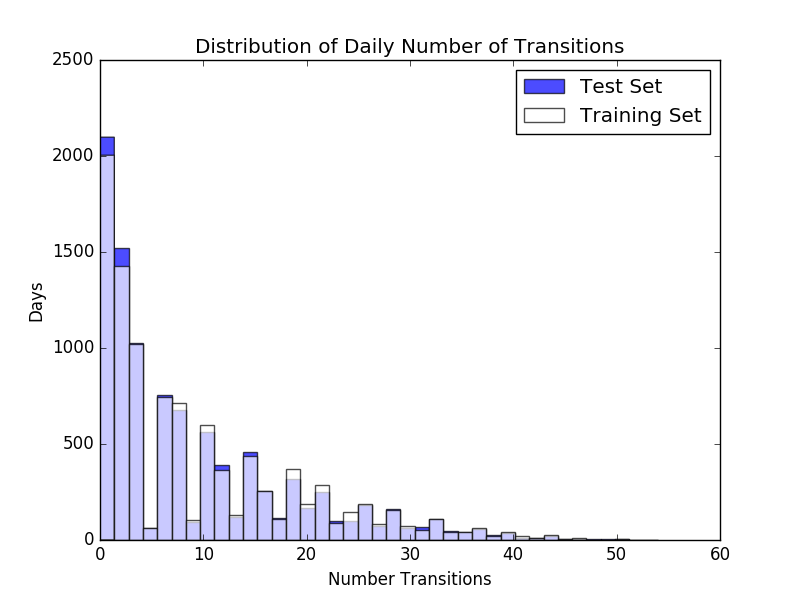
\includegraphics[height = 11cm, width =15cm]{markovTrainTest.png}
 \captionof{figure}{The distribution of number of transitions from training set and testing set. Sample size 10000 user days each. The light blue regions are overlaps of both sets.}
\end{Figure}

The training data used to generate the Markov transition probability matrix has a similar distribution as the testing data.

Despite the Markov generated set and the testing set having similar transition probability matrices, the Markov chain failed to capture the exponential distribution. Because the fixed transition probability matrix was used to generate all data for the Markov chain, we expected a more normally distributed number of transitions transitions, whereas the real data include users that have larger variance in number of transitions. We confirm the concern that a simple three state Markov transition matrix alone does not capture the transition behavior exhibited by the dataset.

\subsection{Aspects of Modeling where Markov Chain Falls Short}
%DONE
We do not believe that such modeling captures user behavior well enough for the following reasons.

\begin{itemize}
\item
Loss of information by the probability matrix.

By categorizing the user into one of the three states, we assume the transition only depends on the number of networks a user is on. The user's likelihood to make a transition can depend on other factors, such as the time of the day. If more users access the network during the daytime, it is plausible that the transition probabilities during the day may be higher than at night.

\item
Loss of individuality of users

The entire dataset contains users of various habitual patterns. There could be a number of groups of users who have contrasting transition probability matrix. By combining all users together, we only gain insight on how an "average user" behaves like, though this "average user" may be a mix of several exemplary users.

\item
Failure to capture the exponential distribution

The Markov chain generated dataset presented a more normal distribution of transitions, as opposed to exponential distribution in the training and testing dataset. This could be potentially explained by the model not capturing the different types of users.
\end{itemize}

We continue to the next section to evaluate what can be done along those dimensions.


\subsection{Questions that Emerge from Yang Experiment Reproduction}
%DONE
Due to the simplicity of the Markov chain, we can ask several major questions: 

\begin{itemize}
\item
Can the entire user population be separated into groups? How many different groups of users are there? 
\item
How frequently do users transition? What does a typical transition look like? What factors can signal, or affect a transition?
\item
Do users exhibit any periodical behavioral patterns?
\end{itemize}

We first answer the grouping question by utilizing clustering algorithms.


%END
\newpage

\section{Modeling}
In this section, we utilized clustering, regression, neural nets, and probabilistic programming to evaluate and predict the number of sessions a user participates in, and the duration of each session.

\subsection{Clustering Finds Three Groups}
%DONE
A closer inspection at the dataset conceives the idea that we may split users into user groups. The population in the dataset is residents of UMass. This could include professors, students, and other populations whose behavioral pattern are likely different. It would be beneficial for the Markov model to take inference for each one of the groups. 

We used K-means analysis for carrying out the clustering analysis. K-means analysis is a commonly used clustering algorithm that is scalable and fast. A typical implementation of the k-means algorithm needs the user to provide the number of clusters, or $k$. The algorithm then picks the $k$ initial starting centroids for the population, and gradually update the position of centers as the algorithm iterates itself. In Tibshirani\cite{tibshirani}, the optimal number of clusters $k$ can be found using the gap statistic, which finds a statistic to measure the comparison of the compactness of the clusters with a distribution of no obvious clustering. We implemented such an algorithm with features including ID, IP, start time, end time, average session duration, Android, Apple, device, whether the ISP is wireless, whether the ISP is wifi, and average number of sessions per day. Three clusters were identified by the algorithm. This clustering separates the users mainly by average session durations. 

\begin{Figure}
 \centering
 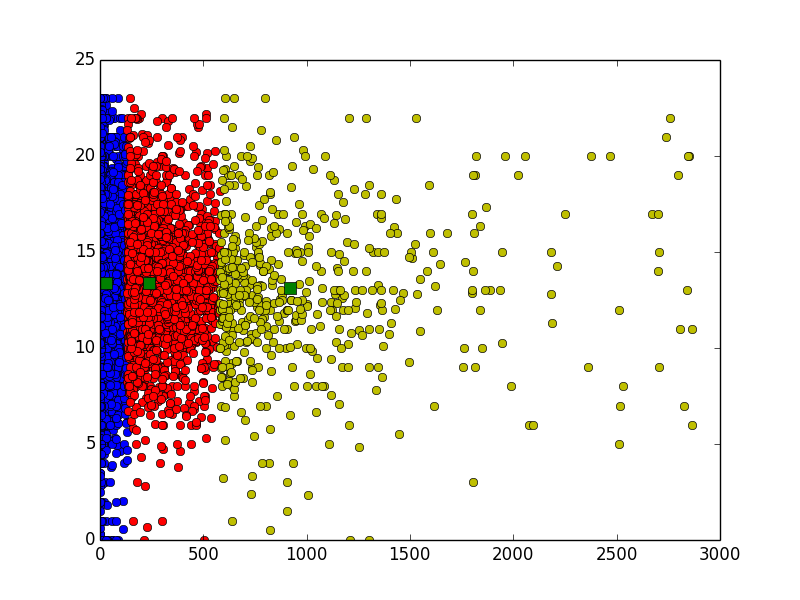
\includegraphics[height = 8cm, width =12cm]{3ClusterKMeans.png}
 \captionof{figure}{The clustering algorithm output. X-axis is average duration in seconds. Y-axis is session start hour. Average duration length significantly affected the clustering. The green dots represent the centers of each cluster.}
\end{Figure}

\begin{Figure}
 \centering
 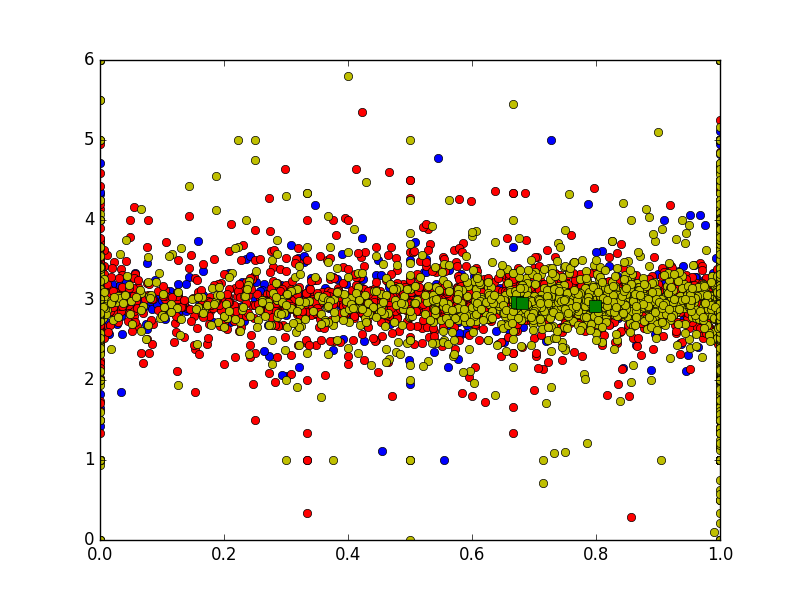
\includegraphics[height = 8cm, width =12cm]{cluterWifiWeekday.png}
 \captionof{figure}{X-axis is portion of user entry generated from a wifi network. Y-axis is day of the week. Those were two of the features that did not significantly affected the clustering.}
\end{Figure}

\begin{Figure}
 \centering
 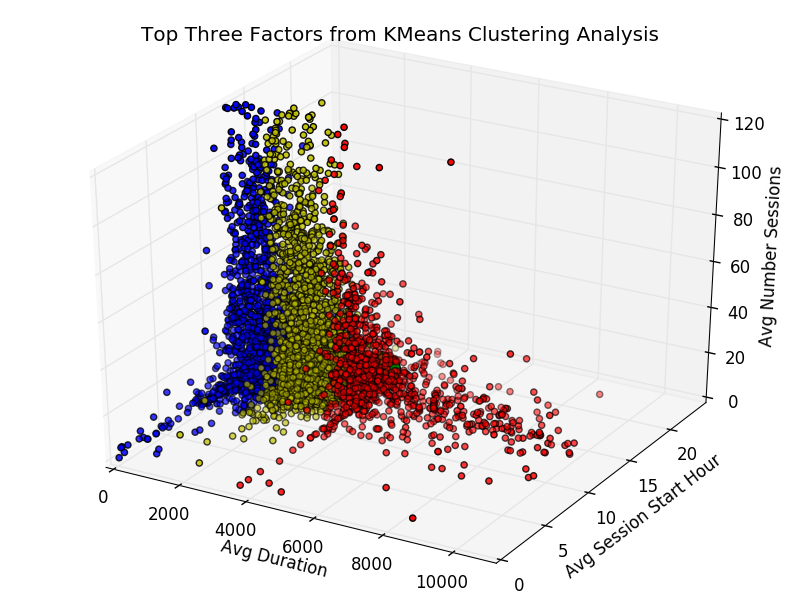
\includegraphics[height = 9cm, width =12cm]{Threefactorclustering.png}
 \captionof{figure}{The K-means clustering algorithm output. The top three factors for separating the dataset are average duration per session, average number of sessions in one day, and the average starting hour for sessions.}
\end{Figure}

The K-means clustering algorithm helps quantify the influence each feature has on dissecting the dataset. Here the k-means algorithm proposes that average session duration is the number one factor for distinguishing user types. Another plausible but less promising factor is the average number of sessions on an average day. 

We note that the clustering output may be less convincing, but it serves as a leading path into potential criteria for distinguishing the users. We make the following arguments and observations regarding this output.

\begin{itemize}
\item
The long duration cluster transitions less frequently.
\item
Users with on average long durations may be less likely to transition. %Have an output graph of a user not 100% utilizing the network
\item
The number of sessions per day can directly affect the calculation of how frequently the user transitions.
\item
Combining the above arguments, we want to verify that users who have on average short sessions and high number of transitions tend to switch between networks more frequently. (Note that a user is not always online, otherwise this claim is trivial. The average online time is roughly 4.5 hours a day\cite{yang}.) This needs to be verified because a user can be on multiple networks simultaneously. Hence when designing a new network catered to mobile users, those users deserve extra attention for congestion.
\end{itemize} 

We move on to test the arguments above. 

\subsection{Clustering Shines Light on Canonical User}

To test out the hypotheses above, we break the users into clusters, and then calculate the Markov transition probability matrix to see whether there is a significant difference.
%%THIS SUBSECTION NEEDS CLARIFICATION AND INCLUSION OF DATA

\begin{center}
    \begin{tabular}{| l | l | l | l |}
    \hline
     Transition Prob.& On 0 Networks & On 1 Network & On $>=1$ Networks\\ 
    \hline
    On 0 Networks Now& 0.930 &0.066 & 0.004\\ 
    On 1 Network& 0.696 &0.266 & 0.038\\ 
    On $>=1$ Networks & 0.291 & 0.356 & 0.353\\
    \hline
    \end{tabular}
\captionof{table}{Empirical estimates of transition probabilities for all users.}
\end{center}

\begin{center}
    \begin{tabular}{| l | l | l | l |}
    \hline
     Transition Prob.& On 0 Networks & On 1 Network & On $>=1$ Networks\\ 
    \hline
    On 0 Networks Now& 0.896 &0.096 & 0.008\\ 
    On 1 Network& 0.694 &0.266 & 0.040\\ 
    On $>=1$ Networks & 0.285 & 0.293 & 0.422\\
    \hline
    \end{tabular}
\captionof{table}{Empirical estimates of transition probabilities for the long duration cluster.}
\end{center}



\begin{hyp}
The average user in the long duration cluster (average duration $\geq67\%$ percentile) exhibits on average less number of transitions than the average user.
\end{hyp}

$H_0$ is that the average user in the long duration cluster exhibits on average the same number of transitions as the average user.

First we see that on average, the long duration users have a daily 18.49 sessions, whereas the average user of the population of 6084 has a daily 20.64 sessions. The result is significant $(p=0.00179)$ by the t-test. So we reject the null hypothesis.

\begin{Figure}
\centering
 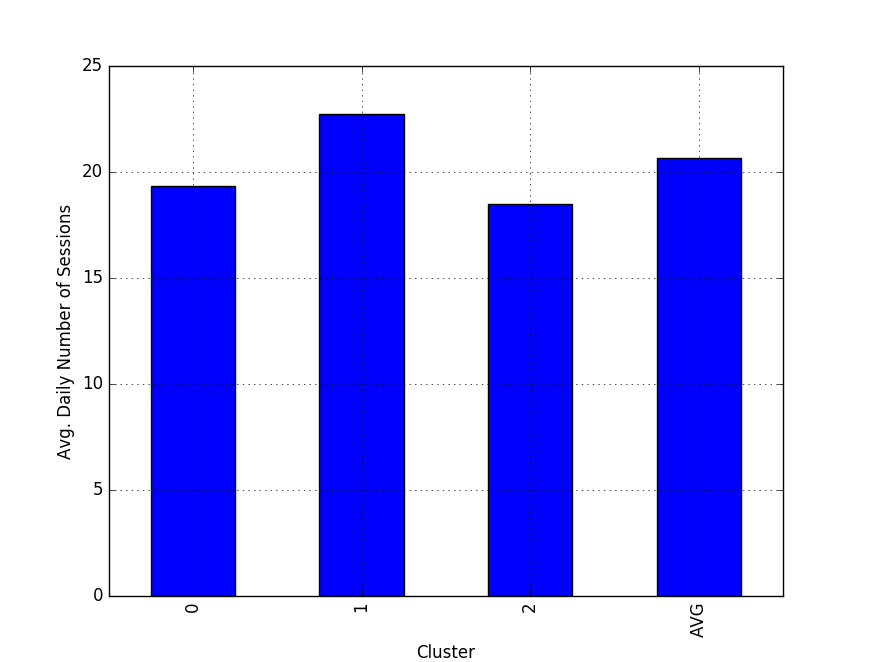
\includegraphics[height = 6cm, width =9cm]{clusteredAVGNUMSESSION.png}
 \captionof{figure}{The average number of sessions per cluster.}
\end{Figure}

\begin{hyp}
Users with on average the most sessions per day (top 33\%) transition more frequently than the average user.
\end{hyp}

By using a similar t-test, we observe that users with more sessions group on average transition more frequently than the average user $(p = 0.00834)$.

\subsection{Regression Helps Weighing Factors}

Another aspect of the Yang model that can be improved and discussed is the assumption that the number of networks the user is on solely determines the transition probabilities. We'd like to quantify the effect other features have on the transitioning.

To answer the question how frequently do users transition, there are several parameters we can model. We chose to model for each user, how many sessions happened in a given day, and what is the duration of each session. If we can accurately model the number of sessions in a day, how long each sessions is, and when exactly these sessions happen, then we can overlay the sessions to evaluate the transitions.

We first tried out with regression analysis. Regression analysis evaluates the relationship between a dependent variable and multiple independent variables. It does so by creating a curve that fits all the data points with minimal total error norm. We started out by exploring linear regression models for simplicity. More specifically, let each $x_i$ be a $p$-dimensional feature vector for prediction, for each $y_i$ the prediction values, a typical regression estimates $\beta$ by minimizing

\begin{equation*}
\sum_{i}{(y_i - x_i^T\beta)^2},
\end{equation*}

where $\beta$ is the weight vector for the variables. 

Regression analysis can be used to discover correlations between the variables. One of the challenges of our dataset is that the predictors are not entirely independent. Hence we tried Ridge regression and logistic regression.


\subsubsection{Ridge Regression}
%FIX THE Ordering for presentation
%Want only prediction of num sessions
%Show duration is not normally distributed in logistic regression
\paragraph{Background}
Ridge regression is a technique that evaluates multiple regression data that suffer from multicollinearity\cite{ridge}, or multiple predictor variables being highly correlated. Ridge regression resolves that issue by \textit{regularization}, or adding a penalty on the weight sizes. Specifically, let each $x_i$ be a $p$-dimensional feature vector for prediction, for each $y_i$ the prediction values, Ridge regression estimates $\beta$ by minimizing

\begin{equation*}
\sum_{i}{(y_i - x_i^T\beta)^2 + \lambda\sum_{j=1}^p{\beta_j^2}},
\end{equation*}

where $\beta$ is the weight vector for the variables, and $\beta_j$ is the weight vector for the $j$th variable. The first sum calculates the error term, and the second sum creates an additional penalty on the absolute size of the individual weights. This partially resolves the multicollinearity of the variables. If two variables are negatively correlated, the additional regularization term pushes the weights to small absolute values\cite{bishop}. Note that there is an additional regularization constant $\lambda$, which controls how much having weight values of small absolute values matters. The choice of $\lambda$ is due to the researcher and trial and error.

\paragraph{Results}
\paragraph{Predicting Number of Sessions}
%% HERE
We first tried to predict the average number of sessions for each day for every user as it is normally distributed. We used scikit-learn\cite{scikitlearn} as our library, for its ease of use and availability of tutorials. We used all 6000 users for our data. We took 60\% of the users as our training set, and 40\% as the testing set. For each user day, we passed in the following features: whether the device is apple, whether the device is android, what day of the week it is, the user's likelihood to be on a cellular network that day, average duration for this user's sessions, average session start time for this user. The prediction score is defined by the $R^2$ score, or

\begin{equation*}
1 - \frac{\sum{(y_{true} - y_{pred} )^2}}{\sum{(y_{true} - \overline{y_{true}}})^2},
\end{equation*}

or how much the model explains the variability in the data around its mean. We did the prediction using 1. The general population. 2. Once for each cluster.

\begin{Figure}
 \centering
 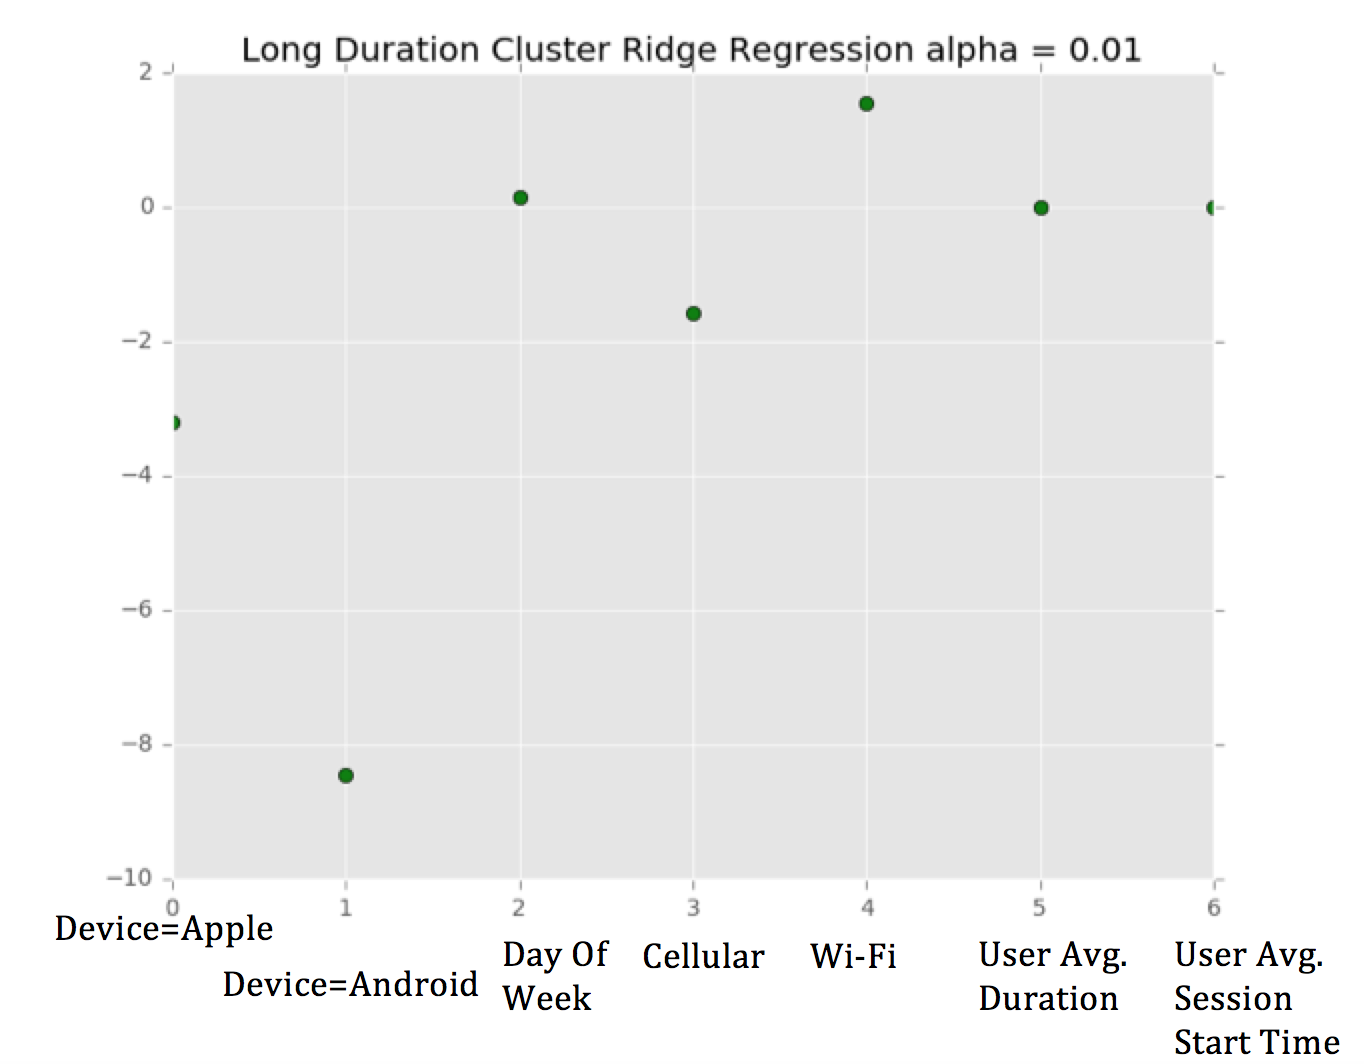
\includegraphics[height = 7cm, width =10cm]{fixedFeatures.png}
 \captionof{figure}{The long cluster average session length prediction. Each integer on the x-axis is a feature and the y-axis is showing the feature's corresponding weight.}
\end{Figure}

$R^2$ scores on the training dataset and testing dataset reach around 7\% for both the general population and each cluster. Training the model took 0.003 seconds on average due to the low dimensions.

The main observations are:

\begin{itemize}
\item
Using just the 7 features, a linear regression model cannot predict the number of sessions in a given day
\item
Being on a cellular network decreases the number of sessions per day. Being on a wifi network increases the number of sessions. This is potentially due to the automatic email checking is only on when on a wifi network to save wireless data usage.
\item
Grouping by cluster does not help show significant difference in prediction accuracy. 
\end{itemize}

Note that in predicting the daily number of sessions, we are no longer accessible to the unique IP address as found in each entry before. This decrease in number of independent variables further decreased the performance of our prediction. 

This result opens up discussion for alternative modeling techniques.


%
%\paragraph{Predicting Session Duration is Difficult}

%First we looked at the general user population. We used scikit-learn as our library, for its ease of use and availability of tutorials. We passed in 5 million entries of session data, where each entry $x_i$ consists of user ID, IP address by bits (32 bits), timeStartBucket \{0 - 23\}, day of week, device, whether the device is Apple, and whether the device is Android. Each $y_i$ is the duration of the session. We used a set of $\lambda$ values $[0, 0.001, 0.01, 0.1, 0.2, 0.5]$. Note that setting $\lambda$ equal to 0 is equivalent to not having regularization. We used the first 2.5 million entries to train the model. We use the model to predict the remaining 2.5 million entries. The prediction score is defined by the $R^2$ score, or


%or how much the model explains the variability in the data around its mean.

%\begin{Figure}
 %\centering
 %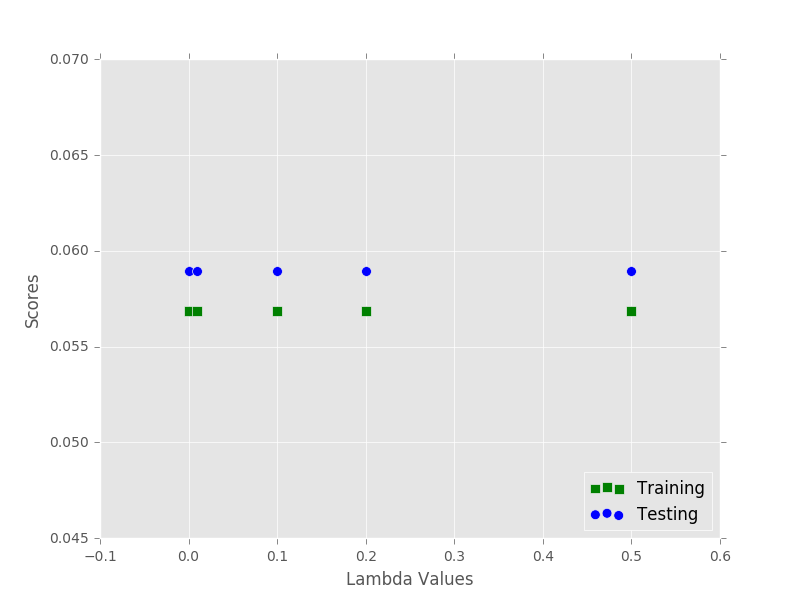
\includegraphics[height = 7cm, width =10cm]{ridgeScores.png}
% \captionof{figure}{Ridge Regression Scores. Lambda values do not significantly affect performance.}
%\end{Figure}

%Using the first 2.5 million entries to train, we tried to make predictions on the session duration of the remaining 2.5 million available entries. Unfortunately, we reached low $R^2$ scores ($<10\%$) on both the training and testing dataset for Ridge regression. 




%The results show that the features we used cannot distinguish whether a duration is going to be less than a minute or an hour long. Because the prediction is linear, the model shows minimal predictive power. We then examined other statistical approaches that can better capture this discontinuous distribution of the dependent variable. See 4.3.2 for logistic regression.



\subsubsection{Logistic Regression}
%THIS Section is fine
\paragraph{Motivation}
Another parameter we'd like to predict is the duration of each session. We first look at the distribution of session durations.

\begin{Figure}
 \centering
 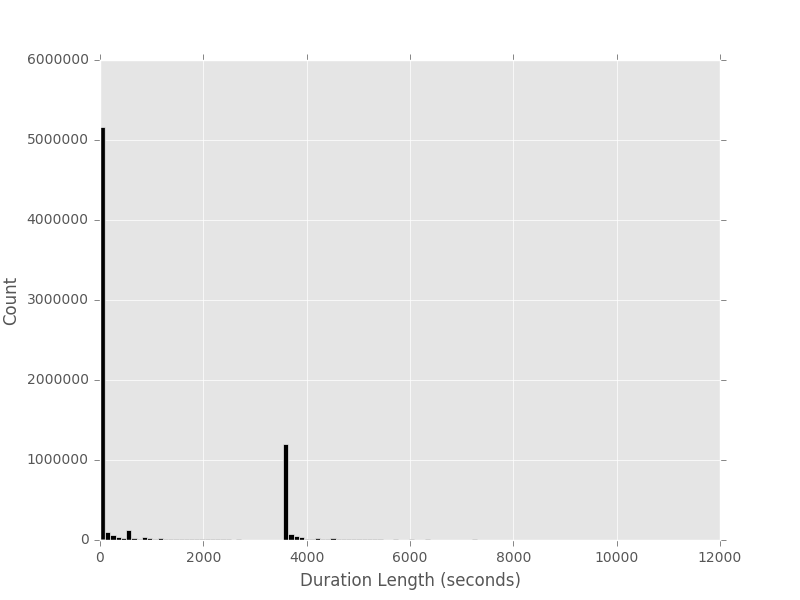
\includegraphics[height = 7cm, width =10cm]{durationDistribution.png}
 \captionof{figure}{The distribution of session durations, in seconds. Note the second peak at the hour mark.}
\end{Figure}

We observe that there is a secondary peak at the hour mark, and more importantly, the distribution is not normal. A deeper inspection at the original processed dataset reveals that the hour peak was largely due to the server closing down connections after an hour of idle time. This does not conflict with our definition of session, as the user was \textit{on}, despite not utilizing the network, for the entire time.

Since Ridge regression assumes a normal distribution, it will not work well directly predicting the session duration. We asked whether a categorical answer (such as long or short) can be acquired through regression. We decided to use logistic regression to give a categorial prediction for session duration.

\paragraph{Background}

Logistic regression is a regression model where the dependent variable is categorical, as opposed to continuous. Logistic regression makes its predictions by comparing the likelihood of each individual category, and picks the category with the highest likelihood.

Formally, the logistic regression tries to predict the conditional probability $Pr(Y=1 | X= x)$, where $Y$ is the binary indicator variable for the category (0 or 1). In order to reach a 0 or 1 output, we need to carefully examine the math to produce the correct results.

The formal model \cite{cmulogisitc} is that

\begin{equation*}
log\frac{p(x)}{1-p(x)} = \gamma_0 + x\cdot \gamma
\end{equation*}

where $\gamma_0$ is the $y$-intercept and $\gamma$ the weights for the features. Solving for $p$ we get

\begin{equation*}
p(x) = \frac{e^{\gamma_0 + x \cdot \gamma}}{1 + e^{\gamma_0 + x \cdot \gamma}} = \frac{1}{1 + e^{-(\gamma_0 + x \cdot \gamma)}}
\end{equation*}

To minimize error, we should predict $Y=1$ when $p \geq 0.5$ and $Y=0$ when $p < 0.5$. This means predict 1 when $\gamma_0 + x \cdot \gamma \geq 0$, 0 otherwise.

We used a variation of the logistic regression model, namely we expanded it to predict from multiple categories. That is,

\begin{equation*}
Pr(Y=c | X = x) = \frac{e^{\gamma_0^{(c)}}+x\cdot \gamma^{(c)}}{\sum_c{e^{\gamma_0^{(c)} + x\cdot \gamma^{(c)}} }}
\end{equation*}

Instead of having one set of parameters $\gamma_0$ and $\gamma$, each class $c$ has its own offset $\gamma_0^{(c)}$ and weight vector $\gamma^{(c)}$. The remaining calculations are analogous as the binary case. The category $c$ with the highest probability gets picked.

\paragraph{Results}

We used scikit-learn\cite{scikitlearn} as our library for its readily implemented multi-class logistic regression module. Because we did not have enough dimensions to capture the distribution, we decided to expand the feature size of the dataset, by including all the bits of the IP address. We passed in 2.5 million entries of session data for training, where each entry $x_i$ consists of user ID, IP address by bits (32 bits), timeStartBucket \{0 - 23\}, day of week, device, whether the device is Apple, and whether the device is Android. We further broke duration into short ( $<$ 5s), mid (5s - 60 mins), and long ( $>$ 60 mins). The cutoff at 60 minutes is because we noticed a peak at slightly more than 60 minutes for duration distributions. We used another 2.5 million session data entries for testing set to predict the duration tag.

\begin{Figure}
 \centering
 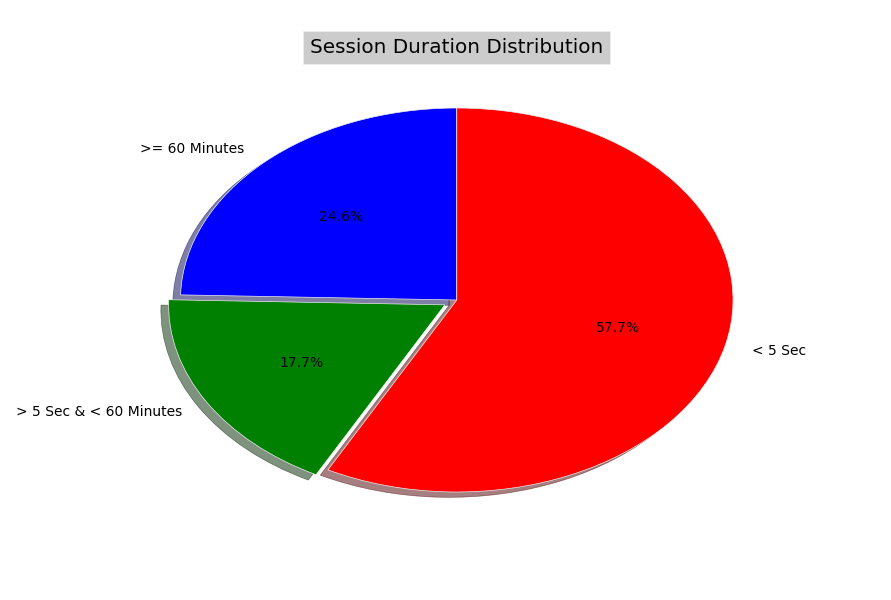
\includegraphics[height = 9cm, width =10cm]{durationDistPie.png}
 \captionof{figure}{The distribution of session durations, by tags.}
\end{Figure}

The logistic regression predicts correctly the duration tag($y_i$=long, mid, or short) at $67\%$ accuracy, which is better than chance (1/3). Note that it also outperforms the simple strategy of always predicting "short" of 58\% accuracy. However, 67\% is far from accurate. The features that carry the most weights are Apple or Android, and specific leading bits of the IP address. Having the device being Android produces more likely a long session. This naturally leads to questions like whether the Android's transfer protocol and app settings by default lets the user stay on a network for long periods of time without disconnection.


%Here a regression model was used to predict the number of sessions of each user per day. Since each user is different, we tried three approaches: 
%\begin{itemize}
%\item
%Treat all users as a uniform group. 
%\item
%Cluster users as user groups.
%\item
%Treat each user as a separate entity.
%\end{itemize}

\subsection{Neural Net Increases Performance}

\subsubsection{Background}

We see that the regression approaches we took have limited practicality as they were either linear or suffered from not enough features. Alternatively, we can fix the number of basis functions but allow them to be adaptive \cite{bishop}.

Neural network is one such approach that allow basis functions to adapt to nonlinear modeling. A neural net is very useful in problem domains where no known function for approximating the given features to their outputs. A neural net contains a collection of layers, where each layer has a collection of nodes. The input features are feed to the first layer and subsequently to next layers to either condense or extract information. The end result is often a classification. The adaptiveness comes from its optimization of the mathematical calculations each round and in the activation functions used.

There are three general types of neural nets depending on the connection architecture of the nets\cite{neuralnetdesign}. 

\begin{itemize}
\item
Feed Forward Network
\item
Recurrent Network
\item
Reinforcement Network 
\end{itemize}

A feed forward network reads the input and feeds forward the information till the output produces a prediction. It is the simplest form of neural net. Such a net is acyclic in the network architecture. A recurrent network, on the other hand, can remember past inputs and forms a directed cycle in the network architecture. A recurrent net is useful in problem domains of natural language processing, in which the earlier part of the sentence is important in deciphering the meaning. A reinforcement network does not directly take input, but takes actions based on its environment and the reward function. Such an approach is often used in the robotics world.

\begin{Figure}
 \centering
 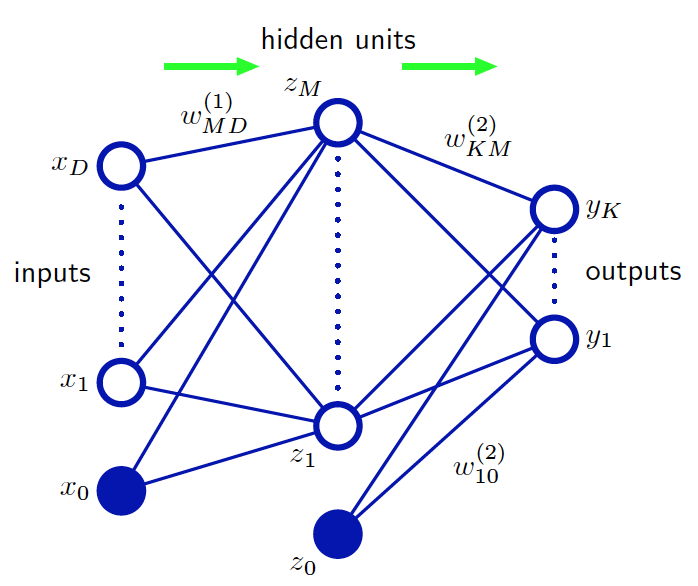
\includegraphics[height = 8cm, width =10cm]{neuralnet.png}
 \captionof{figure}{A one hidden-layer feed forward neural net. Image courtesy to Bishop\cite{bishop}.}
\end{Figure}

\paragraph{Mathematical Background}
The exact way neural networks carry out calculations may be less interesting, so readers can skip this section as needed. The one sentence summary is that each layer of the neural network has an activation function, which can be allowed to be nonlinear, and so multiple layers of such application can adapt to resolve nonlinearity in the dataset.%IMPROVE ONE SENTENCE SUMMARY

Using the notation in the figure above, we have $D$ input data points, each data point $x_i$ contains its feature vector, and $M$ hidden nodes. The notations are due to Bishop\cite{bishop}.

\begin{equation*}
z_j = h(\sum_{i=1}^D{w_{ji}^{(1)}x_i + w_{j0}^{(1)}}),
\end{equation*}

where $h$ is a nonlinear activation function, $w_{ji}$ are the weights for the $i$th input and $j$th hidden node,  $w_{j0}$ is the intercept, or bias, for the $j$th hidden node, and superscripts (1) mean that the parameters are in the first hidden layer. The 

Similar operation happens from the hidden layer to the output layer. The activation function $h$ can be taken as the \textit{sigmoid} function, or

\begin{equation*}
h(a) = \sigma(a)= \frac{1}{1+ e^{-a}},
\end{equation*}

This sigmoid function turns a linear combination of input vectors into a nonlinear output. By taking this activation multiple times, the final output $y_k$ is no longer linearly related to the original input.

\subsubsection{Results and Discussion}

We saw that logistic regression predicted duration tags with 67\% accuracy. We want to increase performance on duration tag predictions, so we implemented a feed-forward neural net with supervised training with one hidden layer.

With aid from Python's TensorFlow\cite{tensorflow} library, we implemented a one-hidden layer feed forward neural net with 7 features, 3 output nodes. We vary the number of hidden nodes from 5, 10, 20, to 30.. The features used were the same as in regression. The activation function is sigmoid and optimization was done using gradient descent. This net correctly predicts the duration tag with 84.5\% accuracy with 20 hidden nodes. The training and prediction took 554 seconds. In general, starting with 10 nodes, increasing the number of nodes no longer increased the prediction accuracy by large amounts.

\begin{center}
    \begin{tabular}{| l | l | l |}
    \hline
     Number of hidden nodes& Prediction Accuracy & Convergence Time\\ 
    \hline%%%%%%
    5 & 57.7\% & 399\\ 
    10 & 83.4\% & 505\\ 
    20 & 84.5\% & 554\\
    30 & 83.6\% & 705 \\
     \hline
    \end{tabular}
\captionof{table}{Comparison of different number of nodes in the hidden layer.}
\end{center}

The results were helpful, but not surprising for the following reasons.

\begin{itemize}
\item
The neural net has more parameters. The 10 hidden parameters created more flexibility for the model to better fit the outcome.
\item
The neural net has a nonlinear activation function. As seen from previous plots, the duration is not linearly correlated with the features given. Hence resolving linearity largely increased performance.
\end{itemize}

%%%%END HERE

\subsection{Bayesian Modeling and Probabilistic Programming}
\subsubsection{Generative vs. Discriminative Modeling}
%Done

Despite the neural net having a high performance, we note that the neural net we used is mostly a classifier. That is, such an algorithm is an example of a discriminative algorithm. In general, modeling algorithms can be classified into two categories, generative vs. discriminative. A discriminative algorithm learns what criteria separate the classes given the dataset.  For instance, logistic regression is a discriminative algorithm. A generative model focuses on each class, and creates a model for what the underlying process for each class is \cite{ng}. Let $x$ be the feature inputs to the model, $y$ be the model output prediction, discriminative models learn $Pr(y | x)$, whereas generative models learn $Pr(x | y)$. That is, given the dataset, how likely is it that the data came from a distribution that is modeled by $y$. Therefore, generative model allows researchers to synthesize new dataset by understanding what the underlying distribution is. The Markov model is a generative approach, whereas regressions and neural nets are mostly descriptive models. We used the the discriminative approach when we needed to correctly classify or quantify parameters. To predict future actions, it is more practical to use a generative approach.

\subsubsection{Probabilistic Programming}
%DONE, unless more model wants to be discussed

In this project we explored modeling using probabilistic programming, which is a type of Bayesian modeling. Bayesian modeling employs a prior belief of how data \textit{could} look like before actually inspecting the dataset. Then, given the dataset, we produce a distribution for each parameter that we are interested in estimating, i.e. the posterior distribution \cite{ppblog}. Probabilistic programming is a way of inferring the ideal parameters for such modeling practice. It is a programming language as it abstracts away the mathematical calculations that goes on in inferencing the optimal parameters, just like a typical programming language abstracts away the storage of pointers in memory.

Roughly speaking, the steps involved in probabilistic programming are as follows:
\begin{itemize}
\item
Declare prior beliefs on what the data looks like.
\item
Feed in dataset.
\item
A sampling algorithm calculates a posterior distribution for each parameter in the model.
\end{itemize}

Probabilistic programming languages enable you to state your priors beliefs and your model with elegant, statistical syntax. Typically, the larger the dataset that's feed in, the less significant the prior beliefs become for learning the final parameters. In rare cases, the initial setup can produce local optimum that is impossible to climb out of. Hence it is recommended to examine several different prior beliefs. 

PP represents data and distributions with probabilistic parameters. Unlike traditional modeling approaches that output exact estimation for their distribution's parameters, a probabilistic programming approach gives estimation for parameters of the distribution in distribution format. For instance, PP may predict "the mean of the duration variable is normally distributed around 3, with a variance of 1.2", as opposed to "the mean of the duration variable is 3". This additional information can better capture the distribution variance and other characteristics of shape, and gives us confidence on whether we picked an appropriate model.

We implemented a five factor model using probabilistic programming. Essentially, we are predicting two things, the number of sessions in a day, and the duration of an average session. We used Python PYMC3 as our API library. PYMC3 uses next-generation Markov Chain Monte Carlo sampling algorithms such as the No-U-Turn Sampler (NUTS) to sample its probability distribution \cite{pymc3}. Essentially, it constructs a Markov Chain that has the desired distribution at its equilibrium distribution, and uses Monte Carlo simulations to reach the approximation equilibrium. We can think of MCMC as similar to gradient descent in neural nets, which is a way of estimating the optimal parameters for the distribution. 

The pros for using PYMC3 include fast inference engine and simplicity to switch between distributions. PYMC3 offers NUTS and Hamiltonian Monte Carlo sampling, which works well on high dimensional and complex posterior distributions and allows complex models to be fit without specialized knowledge on fitting algorithms \cite{pymc3}. For instance, one can easily model the start time for each session as a normal distribution in PYMC3. Later, if one decides that a exponential distribution fits better, s/he can easily specify the desired shape for start time again.

\begin{Figure}
 \centering
 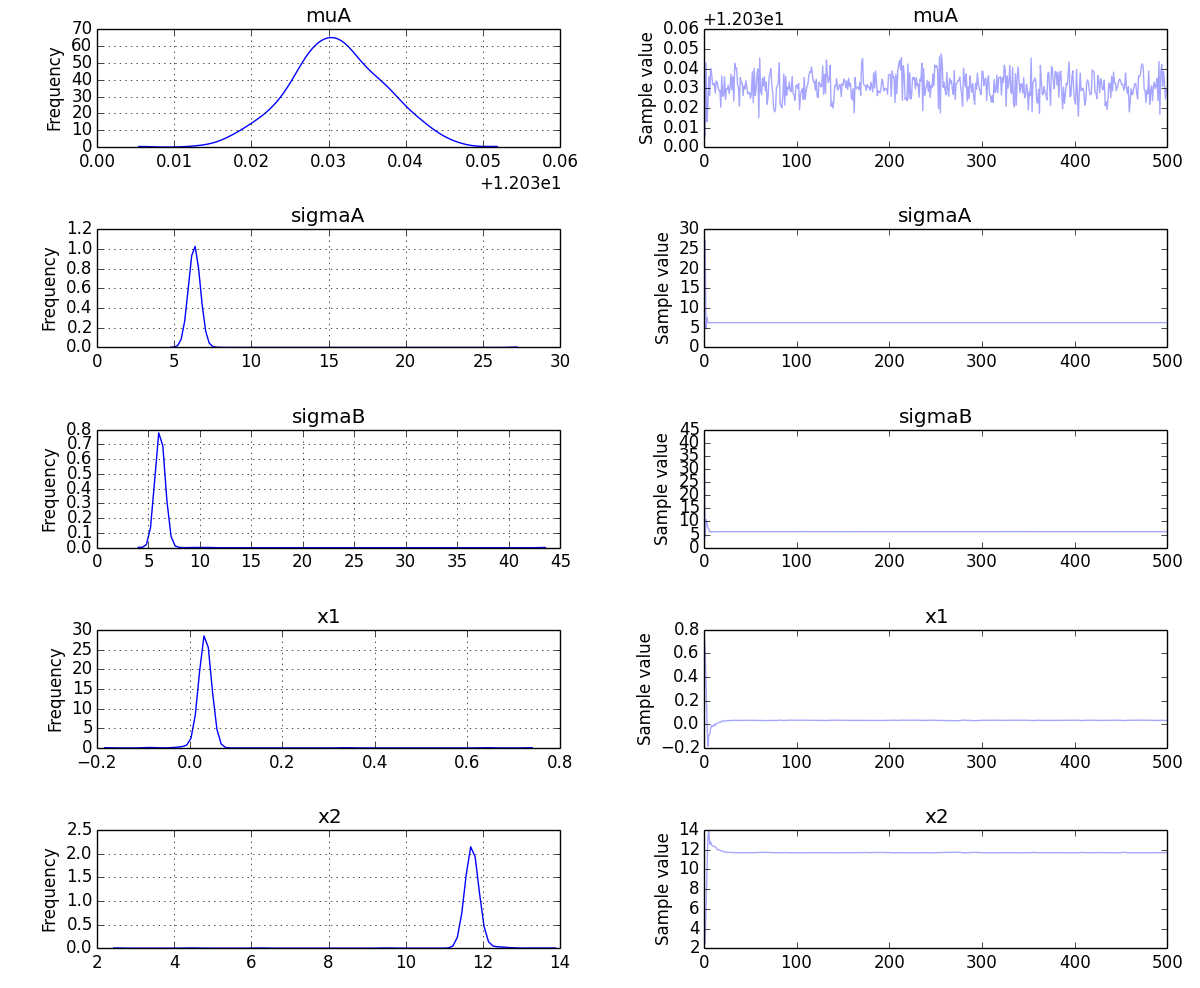
\includegraphics[height = 10cm, width =12cm]{ppsample.png}
 \captionof{figure}{An example PP output using PYMC3. }
\end{Figure}

In the example PP output above, A is the distribution of start times of a typical session, which is modeled as normal. We see that the mean is normally distributed around 12.033 with $\sigma$ of approximately 6. The right column shows each sampled $\mu$ and $\sigma$ values over the 500 sample Monte Carlo trials. The right column also shows convergence of the parameters. We see that the sigma and x-intercept values converged within 20 iterations.

With this approach, we implemented a duration prediction as a combination of two normal distributions, with a switch point. Switch point happened at 1800s, where the later normal has mean 3466 second, the earlier normal has mean 3.53 seconds. This approach is done on the general user population, hence it remains unclear what exactly are the factors that can cause the switch between long and short durations. 

Notably, we spent a lot of time in vain tweaking around the API to analyze more sophisticated, multiply dependent models. Please see the challenges section to see the lessons learnt related to PYMC3 and probabilistic programming.

\paragraph{Summary}
In this chapter, we used various modeling techniques to evaluate some relevant parameters for network transition.

\begin{itemize}
\item
We utilized k-means clustering algorithm to identify three groups for the users.
\item
We used regression to predict the average duration of each session, and to predict the average number of sessions per day for each user.
\item
We used neural nets to predict whether a duration is long, medium length, or short.
\item
We used probabilistic programming to implement a duration distribution estimation as a combination of two normal distribution.
\end{itemize}

\newpage
\section{Approach Comparison}

This project gives the author a much more thorough understanding on what approaches are plausible for a networks dataset. We explored clustering algorithms, regressions, neural nets, and probabilistic programming.

We evaluate the pros and cons of the different approaches along three dimensions: prediction accuracy, speed of convergence, relevance to dataset.

\subsection{Speed}

In general, regressions are the fastest due to the simplicity of its models. A typical logistic regression finishes in less than 30 seconds, whereas training of a million entries in a one-layer feed forward neural net of 10 hidden nodes can take up to 10 minutes. Clustering varies its speed of convergence depending on the exact method. The gap-statistic-enabled K-means algorithm is relatively fast and takes less than a minute to converge. The specific probabilistic programming approach we took only tried to infer the switch point and took relatively short time to converge. In general, because PYMC3 used a Monte Carlo approach as opposed to solving stochastic gradient descent as in neural nets, PP outputs quickly adjust to reach an approximate solution. Neural net remains the slowest approach of all. This is understandable due to hidden layers introducing extra parameters to optimize, and activation calculations introduce additional exponential calculations to be made.

\begin{center}
    \begin{tabular}{| l | l |}
    \hline
     Approach& Real Runtime seconds\\ 
    \hline%%%%%%
    K-means Clustering & 47\\ 
    Ridge Regression & 0.003\\ 
    Logistic Regression& 28\\
    Neural Net & 633\\
    Probabilistic Programming& 15.6\\
    \hline
    \end{tabular}
\captionof{table}{Complexity of different approaches.}
\end{center}

\subsection{Prediction Accuracy}

\begin{center}
    \begin{tabular}{| l | l |}
    \hline
     Approach& Prediction Accuracy\\ 
    \hline%%%%%%
    Ridge Regression & 7\%\\ 
    Logistic Regression& 67\%\\
    Neural Net & 84.5\%\\
    \hline
    \end{tabular}
\captionof{table}{Prediction Accuracy of different approaches.}
\end{center}

We compared prediction on duration for the different approaches. 
 In general, a sophisticated neural net requires a relatively small number of features by compensating with more hidden layers and more nodes in each hidden layer. It also produces the highest output. 

A sophisticated neural net still remains the most fruitful approach. However a neural net decreases the importance of human decision in creating the models. If the human has no idea what is happening in the dataset, then a neural net may better assist him to predict new data points. However, such an approach is difficult to reverse-engineer the reason, and it does not tell causation apart from correlation. Two features may be both positively affecting a tag, but really one of the two causes the other and the positivity of the tag. So, if we use a graphical model approach, i.e. bayesian probabilistic approach, we can more accurately specify the logical dependencies of the features. Regressions in general trade speed for accuracy. 

\subsection{Relevance to Dataset}
Ceteris paribus, we see that neural nets perform the best because it introduces hidden layers and extra parameters. This suggests that in all trainings we did, we did not have enough features and parameters to correctly tune for the results. The fundamental difference in the different approaches we take involve how much we understand the dataset. The specific probabilistic programming toolkit we used requires knowledge on the structure of the dataset. We need to additionally understand the structural dependence of the parameters.

Regressions do not perform as well, as we mostly tried out linear approaches. The more sophisticated logistic regression does well in predicting categorial data, but gets beaten by neural nets.

This is somewhat due to the feature size of our dataset. For each entry, we had at most 10 parameters. Those 10 parameters do not necessarily have enough decision power over the prediction values we wanted to predict. Therefore, a neural net may be a better approach, as it introduces enough hidden parameters. Alternatively, we could introduce hidden intermediate nodes in the graphical models and connect them with corresponding nodes. However, such an approach proves to be overly complex beyond PYMC3 abilities. This alternative approach introduces additional difficulty for us to understand the model. Because we have to specify exactly how the two parameters are related, whether linear, polynomial, exponential, or some other functions, we can understand the model better, but it burdens us to come up with the correct modeling. 

We see that PYMC3 was better at predicting the shape of a given distribution, rather than clarifying hierarchical feature dependence. It is good at picking out the model in the following way: we have several distributions of what the coin's true face probability may look like. We want to know which model is more likely. We used probabilistic programming to infer using a list of runs, we found out that the coin is most likely fair.

\paragraph{Summary}

We compared and contrasted the various modeling techniques for speed, prediction accuracy, and relevance. We see that the neural net has the highest prediction accuracy, the regression and probabilistic programming methods are fast, and we argued that neural net is an appropriate method for this dataset due to the small number of features.
\newpage

\section{Toolkit}

In this chapter we list and discuss the software we used for carrying out this research. We make arguments on why we picked the specific software, if necessary.

Multiple tools were used in carrying out this research. A quick list gives Python Pandas\cite{pandas}, TensorFlow\cite{tensorflow}, PYMC3\cite{pymc3}, scikit-learn\cite{scikitlearn}. 

We decided to use Python as our main programming language. Python is well accepted for data analysis in the research community and the researchers have mastery on Python.

We decided to use a probabilistic programming approach. The advantage of using probabilistic programming is that the inference engine is readily implemented in the API, as opposed to burden the researchers to implement the inference algorithm from scratch\cite[p.4]{ghah}. This additional time gives researchers more time to explore different models. 

There are many probabilistic programming tools available currently, many under active development. The researcher of this project wanted to pick a tool that has a relatively small learning curve, a stable release and a sophisticated support platform. Hence all separately written programming languages were not out of scope. We chose to use Python PYMC3 for our probabilistic programming API. PYMC3 APIs are easy to pick up. PYMC3 offers many general discrete and continuous distributions, and the option to specify our own distribution.\cite{pymc3} While PYMC3 only supports a set of common inference methods, we argue that although other inference methods could be faster, optimization of speed is of minimal importance in training our relatively small dataset.

There are several alternative Python APIs for probabilistic programming, and we list their pros and cons.

\begin{center}
    \begin{tabular}{| l | l | l | l |}
    \hline
     PP Language& Learning Curve & Alpha Version Software & Support Platform\\ 
    \hline
    PYMC3 & Low &No & Mainly Python, Stackoverflow\\ 
    Stan\cite{pystan}& Low &No & Mainly R, Stackoverflow\\ 
    Venture & High & Yes & Correspondence with developers\\
    Picture & High & Yes & Correspondence with developers\\
    \hline
    \end{tabular}
\captionof{table}{Comparison of various Python probabilistic programming APIs.}
\end{center}

Both PYMC3 and Stan (pyStan) are python APIs, Venture and Picture are new programming languages developed at MIT specifically for probabilistic programming. All softwares are under active development, but PYMC3 has released multiple stable versions since 2013. Stan has been along for equally long, but it's mainly a R interface that has provided a Python package \cite{pymcstan}. Therefore we picked PYMC3 as our probabilistic programming language.

Pandas is a widely accepted data processing API in python data analysis and our researchers have gained previous proficiency in it. TensorFlow and scikit-learn are typical bundles for writing neural nets and regressions in aiding the data analysis. 

\paragraph{Summary}

We discussed the software choices we made throughout the research. All our software packages were based on python. We used pandas for data processing, TensorFlow for neural nets, PYMC3 for probabilistic programming, and scikit-learn for regression.

\newpage
\section{Challenges}

In this chapter we discuss the challenges faced in implementing the software packages and writing the models. We also discuss the limits we found in the dataset. In short, the dimension of the dataset, the vagueness of transition, and the limits to current technology were all challenges we faced in this research.

\subsection{Challenges in the Dataset}

First is the choice of the dataset. The raw dataset is a sequence of IMAP log entries. Please refer to figure 2 for a sample of the typical sample entry. The main challenges faced in the dataset are

\begin{itemize}
\item
Each entry has limited number of features.
\item
Network traffic trace datasets normally provide limited user identity.
\item
Ending time for a session is ambiguous.
\end{itemize}

We had 12 million entries(lines) of sessions, as shown in figure.

\begin{Figure}
 \centering
 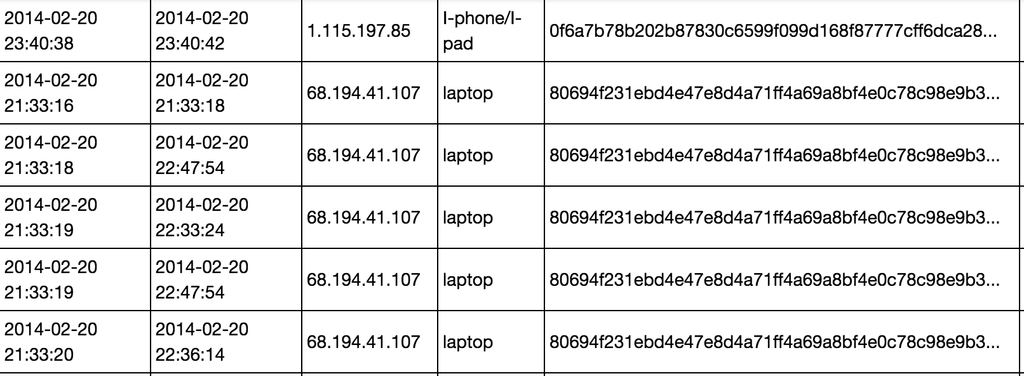
\includegraphics[height = 5cm, width =15cm]{dataSample.png}
 \captionof{figure}{Sample session data, each line is a session. The column headers are session start time, session end time, IP, device, user ID.}
\end{Figure}

This dataset contains many entries, but each entry has a limited number of features, so we went on a pursuit for other relevant features. We included indicator variables for Apple and Android. We included duration of each session, the day of the week, and the city, country, ISP of the IP address. We included an indicator variable for cellular vs. wifi network. Such features were meant to 1. help us achieve higher accuracies in prediction. 2. filter the dataset so that bad data points (missing columns) were dropped. While these variables are relevant, none of them is decisively important for our prediction purposes.

This brings us to the second point that the dataset provides no user identity. This is a tradeoff we had to make. Network traffic traces and email logs are frequently used, but normally do not provide characteristics of users. We used a clustering algorithm to break the dataset into groups, but the algorithm output separates the users by the results of distribution, not by a reasonable feature that gives a less direct answer. It would be more relevant if we can identify the users better prior to clustering. Data such as gender, age, whether s/he is a staff member, years s/he's been on campus can all be beneficial to target the model to a specific user group. For instance, we can test hypotheses such as 1. First year students transition less often (since they are often found in different activity venues). 2. Older population generally transition less (because they have a more fixed routine schedule).

Another particular challenge in this dataset is that the exact ending time for a session is hard to define, unless we see that the connection is reset by peer. In processing our datasets, we made the assumption that a user is on the network unless this network connection is explicitly closed or reset. This can introduce bias for users who were just on the network for a very short period of time but did not detach from the network as seen in logs. We make the argument that from the perspective of network design: since incoming data will still be directed to this idle but attached address, it is reasonable to consider the user as being on the network. This is the tradeoff we had to make for picking this server-side data. It would be difficult to track idle network connections unless we install a client-side application to record when the user actively access the app.

\subsection{Challenges in Technology}
Another aspect of challenge is the technology. In particular, the probabilistic programming toolkit was challenging to maneuver. We chose to use PYMC3 for our API for probabilistic programming because we believed that probabilistic programming allows for flexibility in creating new models, but this API has its limits. 

One can break down ease of changing models in two cases:

\begin{itemize}
\item
How easy is it to add new features?
\item
How easy is it to change the distribution shape of current features?
\end{itemize}

For the API we used, it is easy to change the distribution of a feature, but not so much to add a hierarchically connected feature. In PYMC3, we can easily change the shape of the distribution to binomial, normal, Poisson, etc. due to its general inference engine. The NUTS and HMC sampler can easily readapt to the different shapes that we provide as the inference methods were already tuned. For each distribution class, a specific \textit{logp} method is written to facilitate the parameter estimation gradient calculations in NUTS and HMC sampling. Therefore it is very easy to switch models by means of changing distribution.

\begin{Figure}
 \centering
 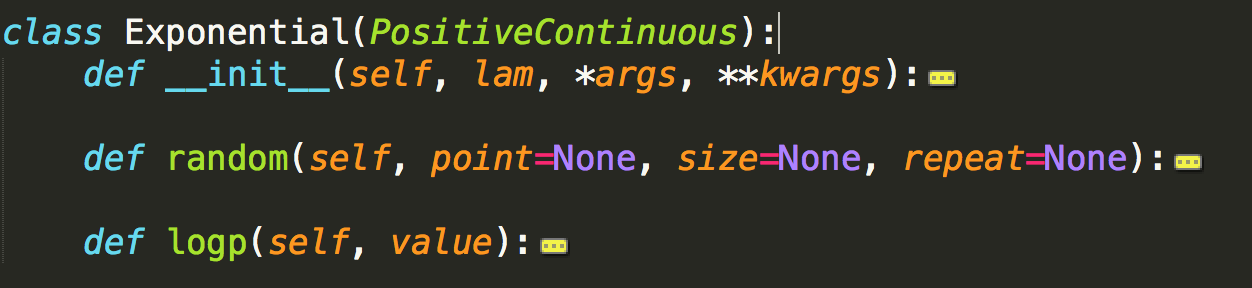
\includegraphics[height = 3cm, width =14cm]{samplePymc.png}
 \captionof{figure}{Exponential distribution implementation in PYMC3.}
\end{Figure}

Many common distributions have readily implemented classes in PYMC3. For each class, a $random()$ method generates samples from this distribution, and a log probability method $logp$ is implemented for fast inference. We can also specify our own distribution by creating a class in this similar format.


It is easy to add new features, as long as the new feature is independent of other features. It is possible to do hierarchical bayesian modeling in PYMC3, but the API was not tuned for hierarchical inference. PYMC3 is meant to help approximate what the true distribution looks like based on feed-in sample data, but not to understand how each feature is affecting the distribution. We wanted to approach the problem by understanding the features' effect on the distribution, using PYMC3. 

We note that there were examples that implemented hierarchically dependent models using PYMC3 \cite{twiecki2}, but the model is minimally hierarchical. We can implement a linear regression using this approach, given the features are independent. If the parameters are dependent themselves, it is in the user's responsibility to figure out which parameter to infer first. If we change one node, we have to rewrite all other variables that is dependent on that node. This tweaking of the API required hacks that slowed down the progress and incurred bugs that were not informative and difficult to fix. For graphical models with multiple-level dependencies, if the user failed to specify the inference order, the inference engine returns errors for not being able to infer hierarchically dependent variables. This is a particular downside of PYMC3, by providing fast inference through Monte Carlo simulations, it sacrifices flexibility in structural dependency. In retrospect, a different API might serve us better in this specific approach we wanted to take. 

On the other hand, in a typical neural network implementation, we can specify an extra feature by adding in another column to the input vector / matrix. Even though the nodes can be dependent themselves, the user does not have to specify them. The actual causal dependence is not resolved, but the correlation will be discovered in the hidden layers, by ways of convolutional layers for dimensionality reduction. Such is not possible in PYMC3. We have to specify the graphical model for the variables first.

Another thing we learnt from applying probabilistic programming techniques is that the model needs to be clearly specified. The human expert needs to know exactly how A and B are linearly, exponentially, or otherwise dependent. In the ideal scenario, once the human feeds in data, the machine understands all the hierarchies and dependencies in data on its own, via a selection of possible dependence functions. This belongs to the field of structural learning, which is a more difficult problem. Tenenbaum \cite{tenenbaum} writes on the current state of hierarchical learning. In short, not only is it doing hill climbing in parameter space, but also in modeling space. The current technology seems to have limited grasp on hierarchical structural learning. 

\paragraph{Summary}
%WRITE SUMMARY for challenges

We discussed two main challenges faced in this research, the dataset and the technology. The main points are

\begin{itemize}
\item
The processed dataset has limited number of relevant features for prediction.
\item
The raw data has ambiguity on when exactly the server closes the connection. 
\item
PYMC3 as an API is good for modeling different shapes of the distribution, but not good for inferencing hierarchically dependent models.
\item
The exact functional relation between the variables needs to be specified in a PYMC3 implementation, which could be tedious.
\end{itemize}


\newpage
\section{Contributions and Conclusion}

\subsection{Contributions}

The contributions of this thesis include 
\begin{itemize}
\item
Evaluated current models and built new models for network topological mobility.
\begin{itemize}
\item
Evaluated Markov chain models to identify areas of improvement
\begin{itemize}
\item
Markov chain produced normal distributions of daily transitions, as opposed to exponential distribution in real data.
\item
Markov chain failed to capture the effect of other features.
\end{itemize}
\item
Utilized k-means clustering algorithm with gap-statistic to acquire three clusters of users, mainly separated by duration distribution.
\item
Evaluated network mobility by user clusters. Implemented Markov transition probability matrices for each cluster.
\end{itemize}
\item
Use and demonstration of a suite of tools for broad exploration possibility.
\begin{itemize}
\item
Exploration of new modeling techniques and their application to networking challenges.
\item
Probabilistic programming to model the duration distribution as a combination of two independent normal curves.
\item
Ridge regression with 7 features to predict average number of sessions. Experimented with various regularization constants.
\item
Logistic regression with 38 features to predict duration tags.
\item
One layer feedforward neural net with 7 input nodes to predict durations tags. Experimented with various number of hidden nodes. 
\end{itemize}
\item
Compared and contrasted the different techniques and tools used in the process.
\item
Neural net has the highest prediction accuracy.
\item
Probabilistic programming and regressions are fast.
\item
PYMC3 is more suitable for models that need different shapes of distribution, rather than resolve feature dependency.
\end{itemize}

\subsection{Conclusion}

Data analysis needs maturity and experience. By doing this project, we have acquired a much deeper understanding of the procedures and priorities of data analysis. The approaches taken to understand a dataset might be limited by the tools and dataset we have, but a good researcher can point the research in an insightful direction. Machine learning algorithms and statistical approaches can help provide additional understanding to the dataset if the researcher knows what factors are important but just don't know how exactly the factors are related. The first step in tackling a data analysis project is to understand what exactly to model for. Then, what exactly are the features that matter. Lastly, we pick the appropriate tools to explore. 

The takeaway lessons in carrying out this thesis project are

\begin{itemize}
\item
Start by understanding what data looks like. Evaluate whether the data distribution looks reasonable. Decide whether to use the data or not.
\item
Compare and contrast various approaches for the purpose of the prediction. Proceed with modeling.
\item
Find aspects the model does not capture and recurse. 
\item
When faced with difficulties in modeling, take a step back and understand the limits of the models. Understand what we know about the dataset and what we want the model to help us find. 
\end{itemize}

%ADD MORE

\newpage

\begin{thebibliography}{25}
\bibliographystyle{plain}
  
\bibitem{beverly} \author{Beverly, Robert}. 2008. {\em Statistical Learning in Network Architecture}. Ph.D. Dissertation. Massachusetts Institute of Technology. 

\bibitem{ghah}\author{Zoubin Ghahramani}. {\em Probabilistic machine learning and artificial intelligence} Nature, 28 May 2015.

\bibitem{jacobson} \author{Jacobson, Van}. 2009. {\em Networking Named Content}. Retrieved May 21, 2016, from http://conferences.sigcomm.org/co-next/2009/papers/Jacobson.pdf

\bibitem{ng}\author{Ng, Andrew}. 2001. {\em On Discriminative vs. Generative classifiers: A comparison of logistic regression and na{\"i}ve Bayes.} Retrieved May 21, 2016, from https://papers.nips.cc/paper/2020-on-discriminative-vs-generative-classifiers-a-comparison-of-logistic-regression-and-naive-bayes

\bibitem{yang}\author{Yang, Sookhyn}. 2015. {\em  Measurement and Modeling of User Transitioning Among Networks.} Retrieved May 21, 2016, from https://people.cs.umass.edu/$\sim$shyang/paper/Yang\_Infocom15.pdf

\bibitem{kulkarni} \author{Kulkarni}. 2015. {\em Picture: A Probabilistic Programming Language for Scene Perception.} Retrieved May 21, 2016, from http://dspace.mit.edu/openaccess-disseminate/1721.1/96620

\bibitem{find}\emph{NSF NeTS FIND Initiative}. Retrieved May 21, 2016, from http://www.nets-find.net/

\bibitem{pymc3} PyMC3. Retrieved May 21, 2016, from https://github.com/pymc-devs/pymc3

\bibitem{tenenbaum} \author{Tenenbaum, Joshua. et al}. 2011. {\em How to Grow a Mind: Statistics, Structure, and Abstraction.} Science, 331(6022), 1279-1285. doi:10.1126/science.1192788

\bibitem{tibshirani} \author{Tibshirani, Robert. et al}. 2001. {\em Estimating the Number of Clusters in a Data Set via the Gap Statistic.} Journal of the Royal Statistical Society: Series B (Statistical Methodology) J Royal Statistical Soc B, 63(2), 411-423. doi:10.1111/1467-9868.00293

\bibitem{ppblog} \author{Finkelstein, Noam}. {\em Probabilistic Programming for Anomaly Detection.} Retrieved May 21, 2016, from http://blog.fastforwardlabs.com/post/143792498983/probabilistic-programming-for-anomaly-detection

\bibitem{pymcstan}\author{Carpenter, Bob}. {\em You'll never guess what's been happening with PyStan and PyMC.} Retrieved May 21, 2016, from http://andrewgelman.com/2015/10/15/whats-the-one-thing-you-have-to-know-about-pystan-and-pymc-click-here-to-find-out/

\bibitem{whyonlyus}\author{Berwick, Rob. Chomsky, Noam}. 2016. {\em Why Only Us: Language and Evolution.} MIT Press.

\bibitem{mobilityfirst}\author{Raychaudhuri, Dipankar}. {\em MobilityFirst Future Internet Architecture Project
Overview}. Retrieved May 21, 2016, from http://mobilityfirst.winlab.rutgers.edu/

\bibitem{netsfia}{\em NSF Future Internet Architecture Project}. Retrieved May 21, 2016, from http://www.nets-fia.net/

\bibitem{pporg} {\em Probabilistic programming}. Retrieved May 21, 2016, from http://probabilistic-programming.org/wiki/Home

\bibitem{markov}\author{Kaelbling, Leslie. et al}. 1998. {\em Planning and acting in partially observable stochastic domains}. Artificial Intelligence, 101(1-2), 99-134. doi:10.1016/s0004-3702(98)00023-x

\bibitem{clustering} {\em scikit-learn 0.17.1 documentation}. Retrieved May 21, 2016, from http://scikit-learn.org/stable/modules/clustering.html

\bibitem{ridge} {\em NCSS Statistics Software Ridge Regression}. Retrieved May 21, 2016, from http://www.ncss.com/wp-content/themes/ncss/pdf/Procedures/NCSS/Ridge\_Regression.pdf

\bibitem{bishop} \author{Bishop, Christopher}. 2006. {\em Pattern Recognition and Machine Learning}. New York: Springer.

\bibitem{cmulogisitc} \author{Faraway, Julian}. 2006. {\em Extending the Linear Model with R}. Boca Raton: Chapman \& Hall/CRC.

\bibitem{neuralnetdesign} \author{Hagan, Martin}. 1996. {\em Neural Network Design}. Boston: PWS Pub.

\bibitem{kmeanscomplexity} \author{Inaba, Mary}. 1994. {\em Applications of weighted Voronoi diagrams and randomization to variance-based k -clustering.} Proceedings of the Tenth Annual Symposium on Computational Geometry - SCG '94. doi:10.1145/177424.178042

\bibitem{twiecki2} \author{Elbers, Danne, et al}. 2014, {\em The Best Of Both Worlds: Hierarchical Linear Regression in PyMC3}. Retrieved May 21, 2016, from http://twiecki.github.io/blog/2014/03/17/bayesian-glms-3/

\bibitem{pandas} {\em Pandas: Python Data Analysis Library}. Retrieved May 23, 2016, from http://pandas.pydata.org/

\bibitem{tensorflow} {\em TensorFlow Is an Open Source Software Library for Machine Intelligence}. Retrieved May 23, 2016, from https://www.tensorflow.org/

\bibitem{scikitlearn}{\em Scikit-learn Machine Learning in Python}. Retrieved May 23, 2016, from http://scikit-learn.org/stable/

\bibitem{pystan} {\em PyStan: The Python Interface to Stan}. Retrieved May 23, 2016, from https://pystan.readthedocs.io/en/latest/

\end{thebibliography}

\end{document}
